\documentclass{article}
\usepackage{graphicx}
\usepackage[margin=1.5cm]{geometry}
\usepackage{amsmath}

\begin{document}

\title{Warm-Up 2}
\author{Prof. Jordan C. Hanson}

\maketitle

\section{Quantitative Data in Chapter 1}

\begin{enumerate}
\item In Fig. \ref{fig:hist}, a \textit{histogram} displays an interesting combination of \textit{categorical} and \textit{quantitative} data.  Each category of student is limited by numerical boundaries.  For example, the first category of students are those who completed between 10 and 13 credit hours.  The categories are displayed on the x-axis.  The y-axis contains the number of students that meet the criteria placing them in the category.  \textbf{Answer the following questions about the histogram.}
\item How many total students are there at the college?  That is, what is the total number of students if you sum the categories? \\ \vspace{1cm}
\item How many students take 16 credit hours or less? \\ \vspace{1cm}
\item What is the average number of credit hours taken?  \textit{Be careful:} Think carefully about how you would extract the total number of credit hours first, then divide by the total number of students.
\end{enumerate}

\begin{figure}
\centering
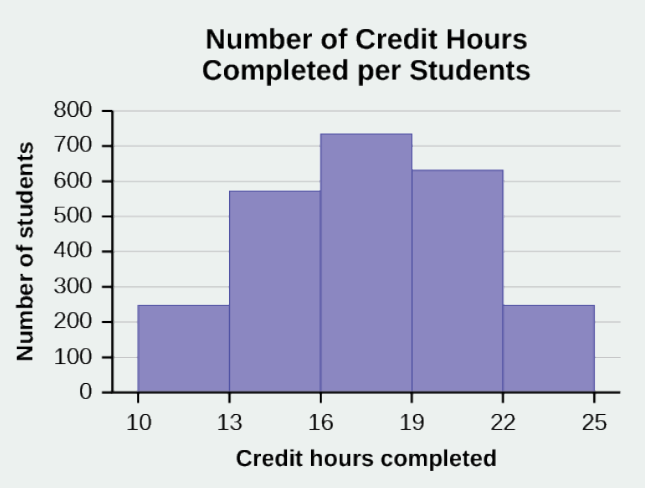
\includegraphics[width=0.4\textwidth]{../figures/histogram.png}
\caption{\label{fig:hist} A \textit{histogram} of the number of credit hours students at a college take.}
\end{figure}

\end{document}
